\documentclass[letterpaper]{article}
\usepackage[utf8]{inputenc}
\usepackage{authblk}
\usepackage{hyperref}
\usepackage{graphicx}
\usepackage{amssymb,amsmath}
\usepackage[usenames,dvipsnames,svgnames,table]{xcolor}
\usepackage[tmargin=3.5cm,bmargin=3.5cm,lmargin=3.5cm,rmargin=3.5cm]{geometry}

\definecolor{blue0}{HTML}{2E81FE}

\hypersetup {
  colorlinks = true, linkcolor = blue0, citecolor = blue0, urlcolor = blue0,
  pdfauthor = {Desjardins-Proulx, Philippe},
}

\renewcommand\Affilfont{\itshape\small}
\setcounter{section}{-1}

\begin{document}

\title{Ecological Interactions and the Netflix Problem}
\author[0,1,2]{Philippe Desjardins-Proulx}
\author[1]{Idaline Laigle}
\author[2]{Timothée Poisot}
\author[1]{Dominique Gravel}
\affil[0]{email: \href{mailto:philippe.desjardins.proulx@usherbrooke.ca}{philippe.desjardins.proulx@usherbrooke.ca}}
\affil[1]{Universit\'e de Sherbrooke, Canada.}
\affil[2]{Universit\'e de Montr\'eal, Canada.}
\date{\today}
\maketitle

\section{Abstract}

Species interactions are key components of ecosystems but we generally have an
incomplete picture of who-eats-who in a given community. Different techniques
have been devised to predict species interactions using theoretical models or
abundances. Here, we explore the $K$ nearest neighbour approach, with a special
emphasis on recommendation. Recommenders are algorithms developed for companies
like Netflix to predict if a customer would like a product given the
preferences of similar customers. These machine learning techniques are
well-suited to ecological interactions, since they focus on positive-only data.
We also explore how the $K$ nearest neighbour approach can be used with both
positive and negative information, in which case the goal of the algorithm is
to fill missing entries from a matrix (imputation). By removing a prey from a
predator, we find that recommenders can guess the missing prey around 50\% of
the times on the first try, with up to 881 possibilities. Traits do not improve
the results for the $K$ nearest neighbour, although a simple test with a
supervised learning approach (random forests) show we can predict interactions
from traits only with high accuracy in the case of positive and negative data.
Recommenders are promising techniques to handle incomplete data-sets in ecology
when no information on traits are available. However, supervised learning
technique are preferable when traits are available. With only a few traits
(body mass and taxonomic distances), it is possible to predict with high
accuracy if two species will interact without any regard to the other species
in the community. This results shows that binary interactions are independant % i.e. binary interactions are weirdly nonecological.
of the ecological community. Further work should focus on developing custom
similarity measures specialized to ecology to improve the $K$NN algorithms,
and using richer data to capture indirect relationships between species.


\section{Introduction}

Species form complex networks of interactions and understanding these
interactions is a major goal of ecology \cite{pim82}. The problem of predicting
whether two species will interact has been approached from various
perspectives. Williams and Martinez \cite{wil00} build a simple theoretical
model capable of generating binary food webs sharing important features with
real food webs, while others have worked to predict interactions from species
abundance data \cite{ade12}. Being able to predict with high enough accuracy
whether two species will interact given simply two sets of attributes, or the
preferences of similar species, would be of value to conservation and invasion
biology, allowing us to build food webs with partial information about
interactions. However, the problem is made difficult by the small number of
interactions relative to non-interactions, and relationships that involve more
than two species.

In 2006, Netflix offered a prize to anyone who would improve their recommender
system by more than 10\%. It took three years before a team could claim the
prize, and the efforts greatly help advanced machine learning methods for
recommenders \cite{mur12}. Recommender systems try to predict the rating a user
would give to an item, recommending them items they would like based on what
similar users like \cite{agg16}. Ecological interactions can also be described
this way: we want to know how much a species would ``like'' a prey.
Interactions are treated as binary variables, two species interact or they
don't, but the same methods could be applied to interaction matrices with
preferences. There are two different ways to see the problem of species
interaction. In the positive-only case, a species has a set of preys, and we
want to predict what other preys they might be interested in. This approach has
the benefit of relying only on our most reliable information: positive
(preferably obseved) interactions. The other approach is to see binary
interactions as a matrix filled with interactions (1s) and non-interactions
(0s). Here, we want to predict the value of a specific missing entry (is
species $x_i$ consuming species $x_j$?).

Statistical machine learning algorithms \cite{mur12} have proven reliable to
build effective predictive models for complex data (the ``unreasonable
effectiveness of data'' \cite{hal09}). We will use a simple technique called
the $K$ nearest neighbour ($K$NN) algorithm both for recommendation (finding
good preys to a species with positive-only information) and matrix imputation
(filling a specific entry in a matrix with positive and negative interactions).
The technique is simple: for a given species, we find the $K$ most similar
species according to some distance (or similarity) measure, and use these $K$
species to base a prediction. For this study, we use a data-set from
\cite{dig14}, which contains 909 species, of which are 881 involved in
predator-prey relationships and 871 have at least one prey. In total, the
data-set has 34 193 interactions. The data also contains 25 binary attributes
for each species, plus their body mass and information on their phylogeny.
We also briefly discuss a supervised learning method, random forests, which is
used to predict an interactions with only the species' traits.

\begin{table}
  \centering
  \begin{tabular}{|lll|}
    \hline
    Method                                 & Input                                    & Prediction \\
    \hline
    \hline
    Recommender (Tanimoto $K$NN)           & Set of traits \& preys for each species  & Recommend new preys\\
    Imputation (Euclidean $K$NN)           & Interaction matrix with missing entries  & Fill missing entries (0s and 1s)\\
    Supervised learning (Random forests)   & Traits (binary and real-valued)          & Interaction (1) or non-interaction (0)\\
    \hline
  \end{tabular}

  \caption{Summary of the three methods used. The first two use the $K$ nearest
  neighbour algorithm, with the Tanimoto distance measure in the positive-only
  case (recommendation), and the Euclidean distance with positive and negative
  values (matrix imputation). The Tanimoto $K$NN makes a recommendation, while
  the Euclidean $K$NN and random forests predict either an interaction or
  a non-interaction. The context for the Euclidean $K$NN and random forests are
  different: the former fill missing entries from a binary interaction matrix
  while the latter makes a prediction based only on the traits of the predator
  and its prey.}

  \label{table:methods_summary}
\end{table}

A summary of the three methods used can be found in table
\ref{table:methods_summary}. The approaches are not directly comparable. For
example, the positive-only $K$NN recommends preys to a species. If we remove a
prey from a species, ask the algorithm to recommend a prey, and check whether
the prey will come up as the recommendation, there are up to 881 possibilities.
On the other hand, the $K$NN algorithm with positive and negative values
(matrix imputation) has to decide whether an entry is an interaction or a
non-interaction, a 50\% chance of success by random. These approaches have
different uses. Positive-only algorithms are interesting because we are rarely
certain that two species do not interact. Also, the $K$NN approach use
information on what similar species do, while random forests only rely
on traits.

We show the $K$NN is particularly effective at retrieving missing interaction
in the positive-only case, succeeding 50\% of the times at recommending the
right species among 881 possibilities. However, the $K$NN algorithm is
significiantly less accurate than random forests to predict an interaction with
positive and negative data. With few traits, the random forests can achieve
high accuracy ($\approx98\%$ for both interactions and non-interactions) without
any information about other species in the community. % This is a really important point.

\section{Method}

\begin{table}
  \centering
  \begin{tabular}{|llll|}
    \hline
    Features          & Abbr. & Description                                                       & $n$ \\
    \hline
    \hline
    AboveGroud        & $AG$   & Whether the species live above the ground.                       & 538 \\
    Annelida          & $An$   & For species of the annelida phylum.                              & 34 \\
    Arthropoda        & $Ar$   & For species of the arthropoda phylum.                            & 813 \\
    Bacteria          & $Bc$   & For species of the bacteria domain.                              & 1 \\
    BelowGround       & $BG$   & For species living below the ground.                             & 464 \\
    Carnivore         & $Ca$   & For species eating other animals.                                & 481 \\
    Crawls            & $Cr$   & Whether the species crawls.                                      & 184 \\
    Cyanobacteria     & $Cy$   & Member of the cyanobacteria phylum.                              & 1 \\
    Detritivore       & $De$   & For species eating detribus.                                     & 355 \\
    Detritus          & $Ds$   & Whether the species can be classifying as a detritus.            & 2 \\
    Fugivore          & $Fg$   & For species eating fruits.                                       & 111 \\
    Fungi             & $Fu$   & Member of the fungi kingdom.                                     & 2 \\
    HasShell          & $HS$   & Whether the species has a shell.                                 & 274 \\
    Herbivore         & $He$   & For species eating plants.                                       & 130 \\
    Immobile          & $Im$   & For immobile species.                                            & 85 \\
    IsHard            & $IH$   & Whether the species has a though exterior (but not a shell).     & 418 \\
    Jumps             & $Ju$   & Whether the species can jump.                                    & 30 \\
    LongLegs          & $LL$   & For species with long legs.                                      & 59 \\
    Mollusca          & $Mo$   & Member of the mollusca phylum.                                   & 45 \\
    Nematoda          & $Ne$   & Member of the nematoda phylum.                                   & 5 \\
    Plantae           & $Pl$   & Member of the plant kinggom.                                     & 3 \\
    Protozoa          & $Pr$   & Member of the protozoa kingdom.                                  & 3 \\
    ShortLegs         & $SL$   & For species with short legs.                                     & 538 \\
    UsePoison         & $UP$   & Whether the species uses poison.                                 & 177 \\
    WebBuilder        & $WB$   & Whether the species builds webs.                                 & 89 \\
    Body mass         & $M$    & Natural logarithm of the body mass in grams                      & 881 \\
    $Ph_0$            & $Ph_0$ & Coordinate on the first axis of a PCA of phylogenetic distances  & 881 \\
    $Ph_1$            & $Ph_1$ & Coordinate on the second axis of a PCA of phylogenetic distances & 881 \\
    \hline
  \end{tabular}

  \caption{The traits used. All traits are binary except for body mass, $Ph_0$,
  and $Ph_1$. We use taxonomy as a proxy of latent traits following
  \cite{mou12}. To do so, we used the R package \emph{ape} to obtain taxonomic
  distances between the species,perform classical multidimensional scaling (or
  principal coordinates analysis \cite{cox01}) on taxonomic distances, and use
  the scores of each species on the first two axes ($Ph_0$ and $Ph_1$) as
  taxonomy-based traits. These three real-valued variables are scaled to be in
  the $[0, 1)$ range. For the Tanimoto similarity index, these three continuous
  variables have to be converted to binary features. For each, we create four
  binary features ($n = 881/4$).}

  \label{table:features}
\end{table}


\subsection{$K$-nearest neighbour}

Both our recommendation and matrix imputation approaches use the $K$-nearest
neighbour ($K$NN) algorithm \cite{mur12}. The $K$NN algorithm is an
instance-based method, it does not build a general internal model of the data,
but instead tries to fill missing entries by a majority vote based on the $K$
nearest (i.e. most similar) entries given some distance metrics. In the case of
recommendation, there is no concept of ``missing entry'', each species is
described by a set of traits and a set of preys, and the algorithm will
recommend new preys to the species based on the preys of its $K$ nearest
neighbours. For example, if $K = 3$, we take the set of preys of the three most
similar species to decide which prey to recommend. If species $A$ is found
twice and $B$ once in the set of preys of the most similar species, we will
recommend $A$ first (assuming, of course, that the species does not already
have this prey). See table \ref{table:tanimoto} for a complete example of
recommendation. In the ``Netflix'' problem, this is equivalent to recommend new
TV series/movies to a user by searching for the users with the most similar
taste and using what they liked as recommendation. It's also possible to
tackle the reverse problem: Amazon uses item-based recommendations, in which
case we are looking for similar items instead of similar users to base our
recommendations \cite{agg16}.

For matrix imputation, if we want to know if our species prey on $A$, we look
at how many of the $K$ most similar species prey on $A$ (a ratio that can be
interpreted as a probability). In this case, the problem is seen as a matrix
with missing entries, so the question is not to recommend new preys to a
predator, but whether a specific relationship exists (see figure
\ref{fig:pearson} for a complete example). It is often suggested to avoid
picking $K$ that are multiple of the number of classes to avoid ties
\cite{the15}. Here there are two classes: interaction and non-interactions, so
we will only use odd $K$s.

Different distance measures can be used. Here, we will use the Tanimoto
coefficient for recommendations and the Euclidean distance for matrix
imputation. Choosing the right value for $K$ is tricky. Low values give high
importance to the most similar entries, while high values provide a larger set
of examples. Fortunately, the most computationally intensive task is to compute
the distances between all pairs, a step that is independent of $K$. As a
consequence, once the distances are computed, we can quickly run the algorithm
with different values $K$.

\subsection{Recommendation}

The Tanimoto (or Jaccard) similarity measure is defined as the size of the
intersection of two sets divided by their union, or:

\begin{equation}
  tanimoto(\mathbf{x}, \mathbf{y}) = \frac{\left\vert\mathbf{x} \cap \mathbf{y}\right\vert}{\left\vert\mathbf{x} \cup \mathbf{y}\right\vert},
\end{equation}

Since it is a similarity measure in the $[0, 1]$ range, we can transform it
into a distance function with $1 - tanimoto(\mathbf{x}, \mathbf{y})$. The
distance function will use two types of information: the set of traits of the
species (see table \ref{table:features}) and their set of preys. We define the
distance function with traits as:

\begin{equation}
  tanimoto_d(\mathbf{x}, \mathbf{y}, w_t) = w_t(1 - tanimoto(\mathbf{x_t}, \mathbf{y_t})) + (1 - w_t)(1 - tanimoto(\mathbf{x_i}, \mathbf{y_i})),
\end{equation}

where $w_t$ is the weight given to traits, $\mathbf{x_t}$ and $\mathbf{y_t}$
are the sets of traits for species $x$ and $y$, and $\mathbf{x_i}$,
$\mathbf{y_i}$ are their sets of preys. Thus, when $w_t = 0$, only interactions
are used to compute the distance, and when $w_t = 1$, only traits are used. See
table \ref{table:tanimoto} for an example.

The data is the set of preys and binary traits for each species (Table
\ref{table:features}). To test the approach, we randomly remove an interaction
for each species and ask the algorithm to recommend up to 10 preys for the
species with the missing interaction. We count how many recommendations are
required to retrieve the missing interactions and compute the top1, top5, and
top10 success rates, which are defined as the probabilities to retrieve the
missing interaction with 1, 5, or 10 recommendations. We repeat this process 10
times for each species with at least 2 preys (7200 attempts). We test all odd
values of $K$ from 1 to 19, and $w_t = \{0, 0.2, 0.4, 0.6, 0.8, 1\}$. We also
divided species in groups according to the number of preys they have to see if
it is easier to find the missing interaction for species with fewer preys.

\begin{table}
  \centering
  \begin{tabular}{|c|ccc|c|}
    \hline
    Species ID  & Traits          & Preys              & Most similar        & Recommendations \\
    \hline
    \hline
    0           & $\{Ar,Ca\}$     & $\{6,42,47\}$      & $\{6,28,70\}$       & $[812, 70, 72]$\\
    \hline
    6           & $\{Ar,Ca\}$     & $\{42,47,70,72\}$  &                     & \\
    28          & $\{Ar,Ca\}$     & $\{42,47,70,812\}$ &                     & \\
    70          & $\{Ca\}$        & $\{42,47,812\}$    &                     & \\
    \dots       & \dots           & \dots              &                     & \\
    \hline
  \end{tabular}

  \caption{Fictional example to illustrate recommendations with $K$ nearest
  neighbour using the Tanimoto distance measure modified to include species
  traits. We are trying to recommend a prey to species 0 given that the three
  most similar species are species 6, 28, and 70. For example, the distance to
  species 70 would be $w_t0.5 + (1 - w_t)1/3$. To find recommendations, the set
  of preys found in the $K = 3$ most similar entries is computed, in this case
  $\{812 = 2, 70 = 2, 72 = 1\}$, leading to the list of recommendations $[812,
  70, 72]$. Because they are found most often in the $K$ most similar species,
  candidates 812 and 70 will be suggested before 72. To test this approach, we
  remove a prey from a species and check whether the algorithm recommend the
  missing prey. Especially with low $K$, it's possible that no recommendations
  can be found, for example if the most similar species has the exact same
  preys.}

  \label{table:tanimoto}
\end{table}

\subsection{Matrix imputation}

The $K$NN algorithm with Euclidean distance works with both positive and
negative entries. In this case, an interaction is represented with a value of
1, while a non-interaction is a represented with 0, in a $n \times n$ matrix
($n = 881$). The goal is to predict the value of a missing entry (Figure
\ref{fig:pearson}). The Euclidean distance is defined as

\begin{equation}
  euclidean(\mathbf{x}, \mathbf{y}) = \sqrt{\sum_i (x_i - y_i)^2}.
\end{equation}

However, we want to give different weights to different aspects of the species,
so we compute the distance between two species as:

\begin{align}
  \Delta_m(\mathbf{x}, \mathbf{y}) &= (w_mmass_x - w_mmass_y)^2,\\
  \Delta_p(\mathbf{x}, \mathbf{y}) &= (w_pp_{0,x} - w_mp_{0,y})^2 + (w_pp_{1,x} - w_mp_{1,y})^2,\\
  \Delta_t(\mathbf{x}, \mathbf{y}) &= \sum_t (w_tt_x - w_tt_y)^2,\\
  \Delta_i(\mathbf{x}, \mathbf{y}) &= \sum_i (w_ii_x - w_ii_y)^2,\\
  euclidean(\mathbf{x}, \mathbf{y}) &= \sqrt{\Delta_m(\mathbf{x}, \mathbf{y}) + \Delta_i(\mathbf{x}, \mathbf{y}) + \Delta_j(\mathbf{x}, \mathbf{y}) + \Delta_j(\mathbf{x}, \mathbf{y})}.
\end{align}

Where $w_m$, $w_p$, $w_t$, $w_i$ are the weight given to body mass, the two
coordinates of a classical multidimensional scaling, binary traits, and
interactions, respectively. For simplicity we require that $w_m + w_p + w_t +
w_i = 1$.

The data is the $881 \times 881$ interaction matrix. To test the $K$NN
algorithm with the Euclidean distance, we randomly remove a single interaction
from the matrix, ask the algorithm to fill the entry, and count how many times
the correct value is retrieved. For each set of parameters tested, we repeat
this process 50 000 times, and count the number of true positives (tp), true
negatives (tn), false positives (fp) and false negatives (fn). The score for
predicting interactions ($Score_y$), non-interactions ($Score_{\neg y}$) and
the accuracy are defined as

\begin{align}
  Score_y &= \frac{tp}{tp + fp},\\
  Score_{\neg y} &= \frac{tn}{tn + fn},\\
  Accuracy &= \frac{Score_y34193 + Score_{\neg y}741968}{881^2},
\end{align}

with 34193 and 741968 being the number of observed interactions and
non-interactions in the 881 by 881 matrix. We also use the True Skill
Statistics (TSS), defined as

\begin{equation}
  TSS = \frac{(tp \times tn) - (fp \times fn)}{(tp + fn)(fp + tn)}.
\end{equation}

The $TSS$ ranges from -1 to 1.

\begin{figure}
  \centering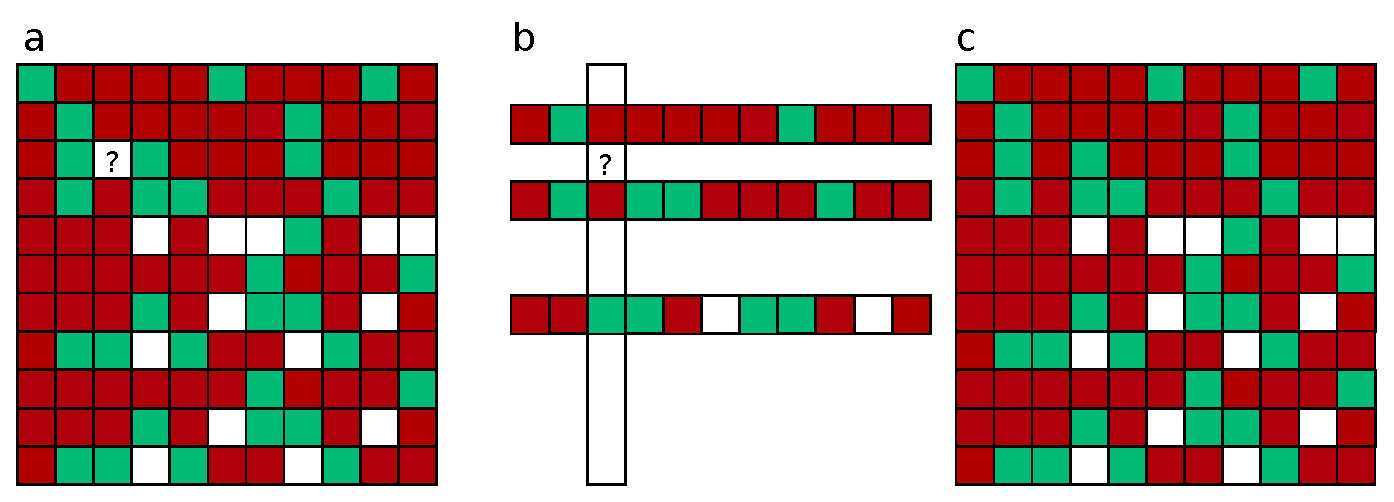
\includegraphics[width=0.85\textwidth]{Figures/pearson.pdf}

  \caption{\textbf{A}: The initial matrix with missing entries, green squares
  are used for interactions, red for non-interactions, and white for missing
  values. Rows represent entries and columns features. In our case, we have a
  square matrix where rows are species and the columns represent their preys.
  We want to find the value denoted by X. \textbf{B}: The K-nearest neighbours
  algorithms look at the entries that are the most similar to the entry with
  the missing value, pick the 3 closest ($K = 3$), and use the values at the
  columns with the missing entry. \textbf{C}: In this case, for the column with
  the missing entry, the 3 nearest neighbours have 2 non-interactions and 1
  interaction, so the algorithm fills the entry with a non-interaction.}

  \label{fig:pearson}
\end{figure}

\subsection{Supervised learning}

We also do a simple test with random forests to see if it is possible to
predict interactions in this dataset using only the traits \cite{bre01b}. In
this case, the random forests perform supervised learning: we are trying to
predict $y$ (interaction) from the vector of traits $\mathbf{x}$ by first
learning a model on the training set, and testing the learned model on a
testing set. We keep 5\% of the data for testing. We perform grid search to
find the optimal parameters for the random forests.

\subsection{Code and Data}

Since several machine learning algorithms depends on computing distances (or
similarities) for all pairs, many data structures have been designed to compute
them efficiently from kd-trees discovered more than thirty years ago
\cite{fri77} to ball trees, metric skip lists, navigating nets \cite{izb15},
and cover trees \cite{bey06,izb15}. We use an exact but naive approach that
works well with small datasets. Since $distance(x, y) = 0$ if $x = y$ and
$distance(x, y) = distance(y, x)$, our C++ implementation stores the distances
in a lower triangular matrix without the diagonal, yielding $n(n - 1)/2$
distances to compute. We used Scikit for random forests \cite{scikit-learn}.
The C++11 code for the $K$NN algorithm, along with Python scripts for random
forests and the data, is available at
\href{https://github.com/PhDP/Articles}{https://github.com/PhDP/Articles}.



\section{Results}

\subsection{Recommendation}

While matrix imputation has a 50\% change of success by random, the Tanimoto
$K$NN needs to pick the right prey among up to 881 possibilities. Yet, it
succeeds on its first recommendation around 50\% of the times. When the first
recommendation fails, the next 9 recommendations only retrieve the right
species around 15\% of the times so the top5 and top10 success rates are fairly
close to the top1 success rate (see figure \ref{fig:tanimoto}). The Tanimoto
measure is particularly effective for species with fewer preys, achieving more
than 80\% success rate for species with 10 or fewer preys (Figure
\ref{fig:tanimoto_n_preys}).

The highest first-try success rates (the probability to pick the missing
interaction on the first recommendation) are found with $K = 7$ and no weights
to traits, and with $K = 17$ and a small weight of 0.2 to traits (Table
\ref{table:tanimoto_k_weights}). Overall, the value of $K$ had little
effect on predictive ability.

\begin{figure}
  \centering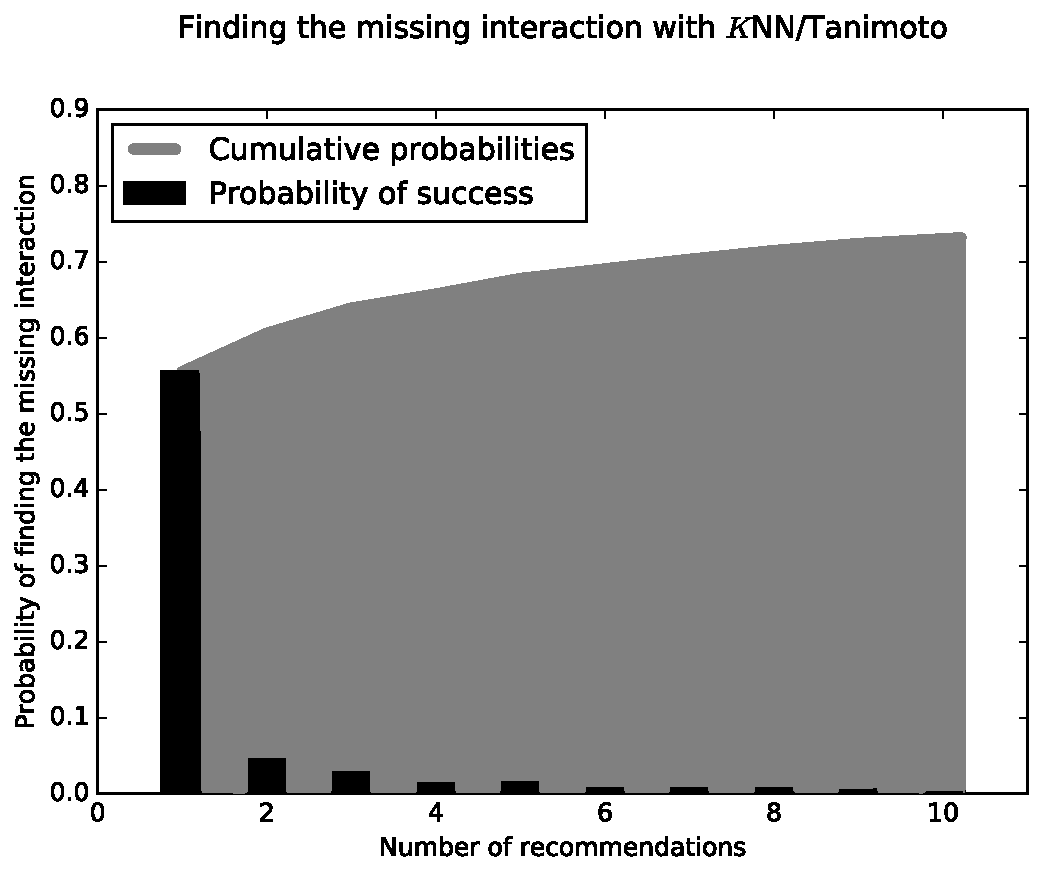
\includegraphics[width=0.85\textwidth]{Figures/tanimoto.pdf}

  \caption{After removing a prey from a predator, we ask the KNN algorithms
  with Tanimoto measure to make 10 recommendations (from best to worst). This
  graphics shows how many recommendations are required to retrieve the missing
  interaction. Most retrieved interactions are found with the first attempt.
  This data was generated with $K = 7$ and $w_t = 0$.}

  \label{fig:tanimoto}
\end{figure}

\begin{figure}
  \centering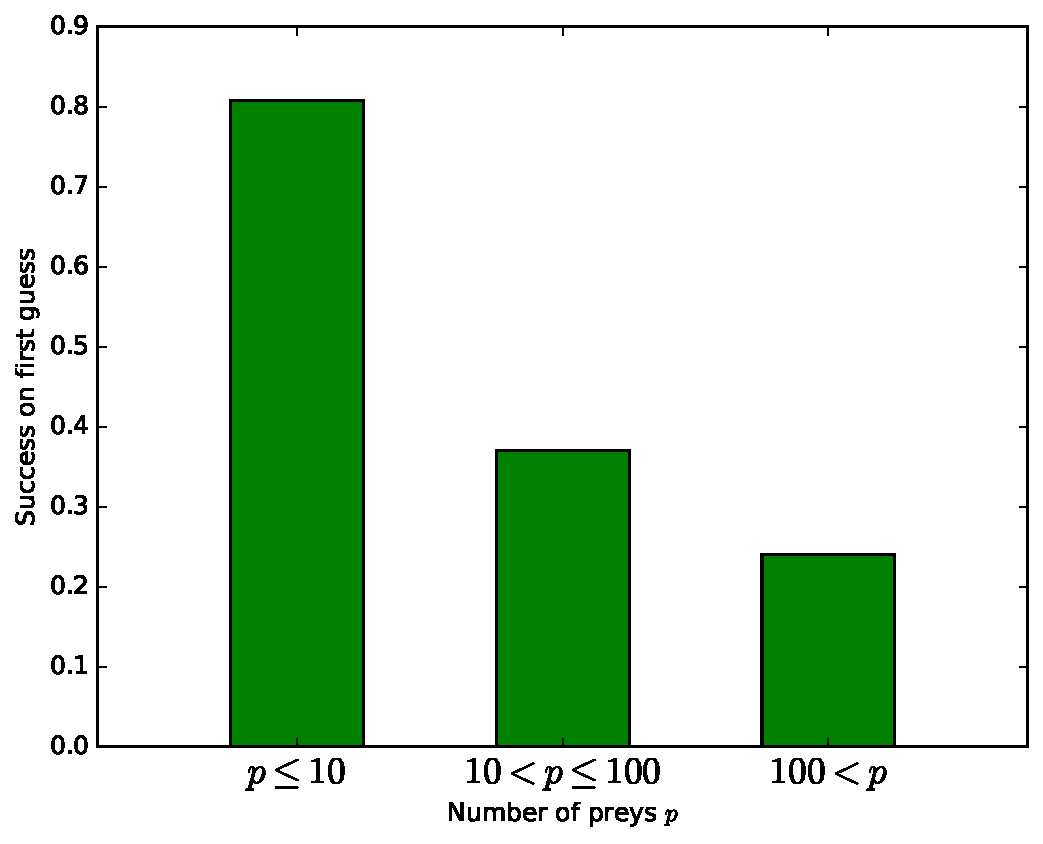
\includegraphics[width=0.85\textwidth]{Figures/tanimoto_n_preys.pdf}

  \caption{Success on first guess with Tanimoto similarity as a function of the
  number of preys. The KNN algorithm with Tanimoto similarity is more effective
  at predicting missing preys when the number of preys is small. This is
  probably in good part because there are more information available to the
  algorithm, since 473 species have 10 or fewer preys, 295 have between 10 and
  100, 103 species have more than 100 preys.}

  \label{fig:tanimoto_n_preys}
\end{figure}

\begin{table}
  \centering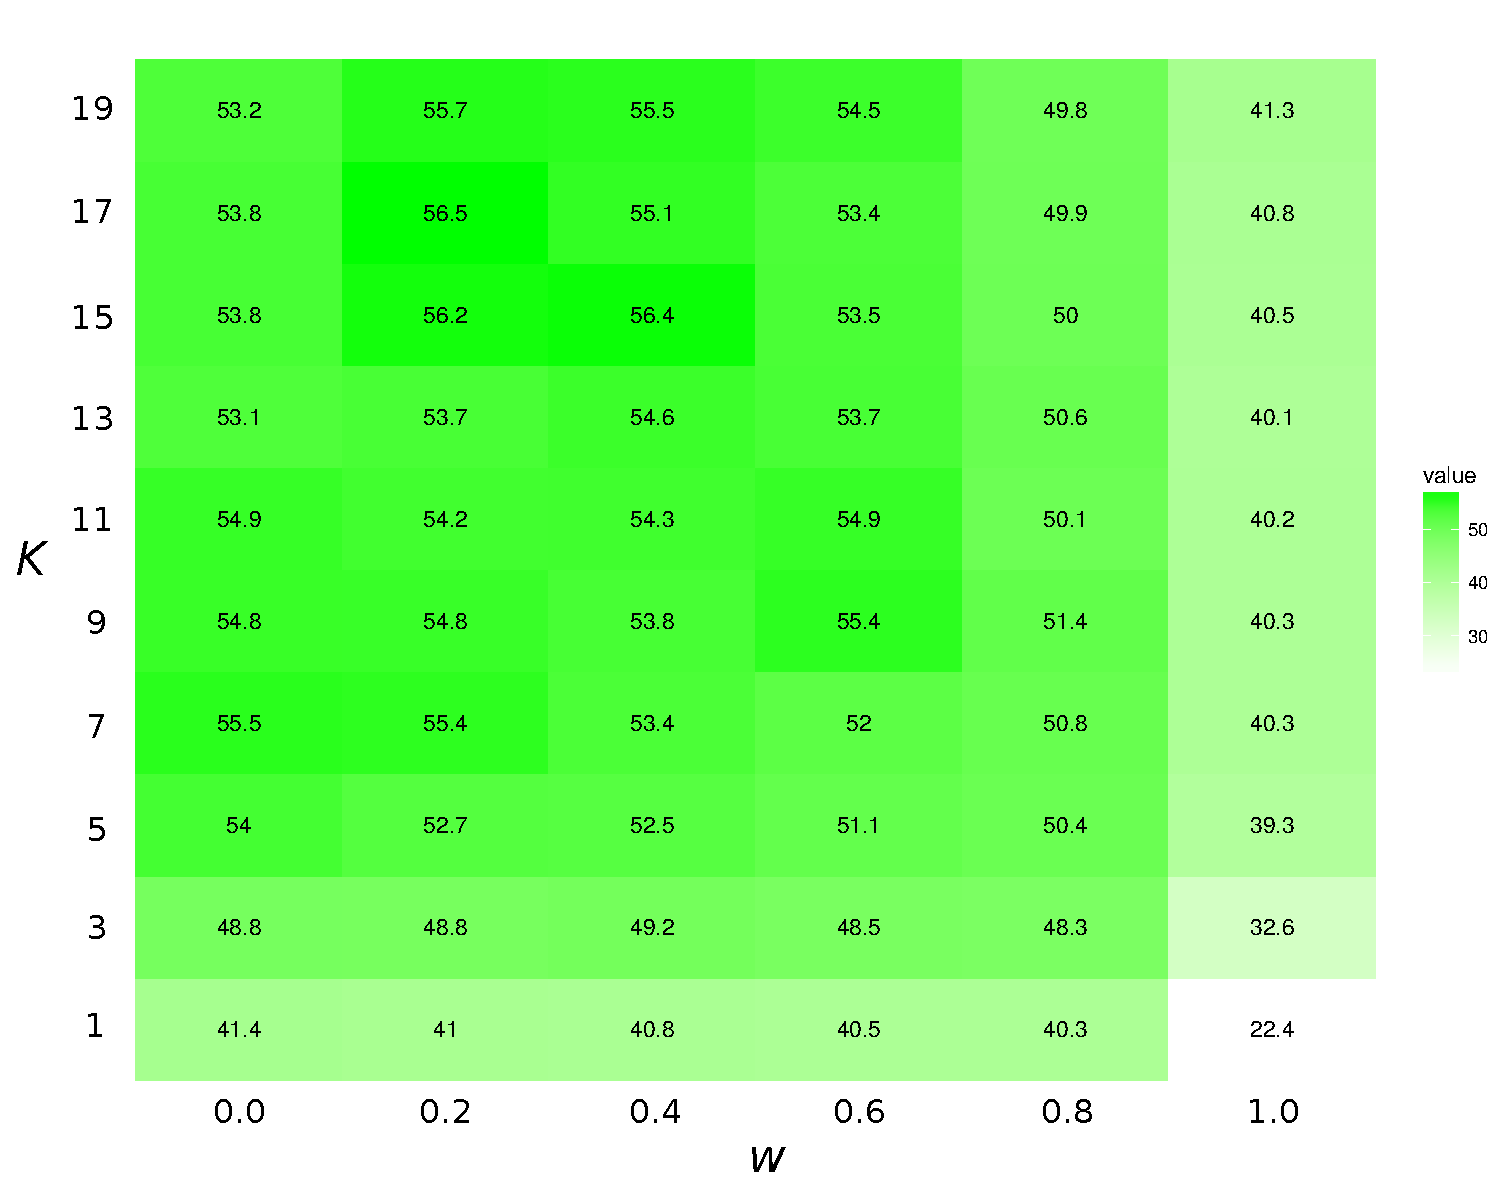
\includegraphics[width=0.85\textwidth]{Figures/r/knn-heatmap.pdf}

  \caption{Top1 success rates for the $K$NN/Tanimoto algorithm with various
  $K$ and weights to traits. When $w_t = 0.0$, the algorithm will only use
  interactions to compute similarity between species. When $w_t = 1$, the
  algorithm will only consider the species' traits (see table
  \ref{table:features}). The value is the probability to retrieve the correct
  missing interaction with the first recommendation. For each entry, $n = 871$
  (the number of species minus 10, the number of species with no preys). The
  best result is achieved with $K = 17$ and $w = 0.2$, although the results
  for most values of $K$ and $w = [0.0, 0.2]$ are all fairly close. The
  success rate increases with $K$ when only traits are considered ($w = 1$).}

  \label{table:tanimoto_k_weights}
\end{table}

\subsection{Matrix imputation}

We show our results with $K$ Nearest neighbours algorithm in table
\ref{table:knn_results}. The best result is achieved with $K = 1$ but has a TSS
of only 0.66 (Table \ref{table:knn_results}). More than 99\% of
non-interactions are predicted correctly, but only $2/3$ of the interactions
are predicted correctly (Table \ref{table:knn_results}).

As for the weights $w_m$ (body mass), $w_p$ (coordinates from a classical
multidimensional scaling of the phylogeny), $w_t$ (binary traits), $w_i$
(interactions), the optimal values for $w_m$ and $w_i$ lie between $1/3$ and
$1/4$ and vary a bit with different values of $K$. $w_t$ has a small but
consistent effect: changing the weight from 0 to $1/3$ improves the result by
roughly 1\%, but higher values will start to decrease predictive ability.
Positive values of $w_p$ always have a negative effect on predictive abilities.
With minor variations with $K$, the optimal weights are thus $w_m \approx 1 /
3$, $w_p = 0$, $w_t = 1 / 3$, $w_i \approx 1 / 3$. With higher $K$, the optimal
weight to $w_i$ increases.

\begin{table}
  \centering
  \begin{tabular}{|c|cccc|}
  \hline
  K                 & $Score_y$ & $Score_{\neg y}$ & Accuracy & TSS \\
  \hline
  \hline
  1                 & 0.6726    & 0.9939            & 0.9804   & 0.6664 \\
  3                 & 0.6277    & 0.9962            & 0.9807   & 0.6239 \\
  5                 & 0.5671    & 0.9975            & 0.9794   & 0.5645 \\
  7                 & 0.5232    & 0.9978            & 0.9780   & 0.5210 \\
  9                 & 0.4754    & 0.9984            & 0.9765   & 0.4739 \\
  \hline
  \end{tabular}

  \caption{Matrix imputation with Euclidean distance. This tables uses the
  weights $w_m = 1/3, w_p = 0, w_t = 1/3, w_i = 1/3$.}

  \label{table:knn_results}
\end{table}

\subsection{Supervised learning}

Random forests predict correctly 99.55\% of the non-interactions and and
96.81\% of the interactions, for a TSS of 0.96. Much of this accuracy is due to
the three real-valued traits (body mass, $Ph_0$, $Ph_1$). Without them, too
many entries have the same feature vector $\mathbf{x}$, making it impossible
for the algorithm to classify them correctly. Removing the binary traits has
little effect on the model. With only body mass, $Ph_0$, $Ph_1$, the TSS of
the random forests is 0.94.

\section{Discussion}

We applied the $K$ nearest neighbour algorithm to the problem of predicting
species interactions with a positive-only (recommendation) approach and by
matrix imputation. Recommendation is arguably a better fit for binary species
interactions, since it is essentially the same problem commercial recommenders
such as Netflix face: given that a user like item $i$, what is the best way to
select other items the user would like. In this case, users are species, and
the items are their preys, but the problem is the same. In both cases, we have
positive evidence but observing with little solid knowledge about
non-interactions. The approach yields strong results, with a top1 success rate
above 50\% in a food web with up to 881 possibilities. The approach could be
used, for example, to reconstruct entire food webs using global database of
interactions. The method's effectiveness rely on nestedness: how much species
cluster around the same set of preys in a food web \cite{gui06}. Thus, it
should be less effective in food webs with more unique predators.

Matrix imputation with $K$NN is less impressive. While it should benefit from
having real-values variables instead of binary traits, the approach clearly
lags behind what a simple supervised learning algorithm can do. The $K$NN
algorithm falls into the realm of unsupervised learning, where the goal is to
find patterns in data \cite{mur12}. The other class of machine learning
algorithms, supervised learning, have the clearer goal of predicting a value
$y$ from a vector of features $\mathbf{x}$. For example, in supervised
learning, we would try to predict an interaction $y$ from the vector of traits
$\mathbf{x}$, while our unsupervised approach allow us to fill entries from an
incomplete matrix regardless of what the entry is (interaction or trait). For
matrix imputation, the $K$NN yields less than impressive results, but our
random forests test on the same dataset achieves a TSS of 0.96 using the binary
traits, body mass, and the coordinates of the classical multidimensional
scaling. A random forest can build effective predictive models by creating
complex rules based on the traits, while the $K$NN algorithm relies on a
simplistic distance metrics. However, the $K$NN approach has some advantages
over supervised learning, namely the capacity to fill any entries from an
interaction matrix and use the information from a species' interactions. The
solution is likely to \emph{learn} distance metrics \cite{bel15} instead of
using a fixed formula. This would allow complex rules while maintaining the
$K$NN's ability to fill arbitrary matrices.

Learning distance metrics is a promising avenue to improve our results. Much
efforts on the Netflix prize focused on improving similarity measures
\cite{tos08,hon06}, and custom similarity metrics can be used to improve
unsupervised classification algorithms \cite{bel15}. Learning distance metrics
from data is a common way to improve methods based on a nearest neighbor search
\cite{xin03,bel15}, allowing the measure itself to be optimized. We only used
the $K$ nearest neighbour algorithm for unsupervised learning, but several
other algorithms can be used to solve the ``Netflix problem''.  For example:
techniques based on linear programming, such as recent exact methods for matrix
completion based on convex optimization \cite{can09} or low-rank matrix
factorization. The latter method reduces a matrix to a multiplication between
two smaller matrices, which can be used both to predict missing entries and to
compress large matrices into small, more manageable matrices \cite{van13}.
Given enough data, deep learning methods such as deep Boltzmann machines could
also be used \cite{zha11}. Deep learning revolutionized machine learning with
neural networks made of layers capable of learning increasingly detailed
representations of complex data \cite{hin06}. Many of the most spectacular
successes of machine learning use deep learning \cite{mni13}. However, learning
several neural layers to form a deep networks would require richer data-sets.

The low sensibility to $K$ in recommendations compared to imputation is
interesting. This is cause by the fact that, as $K$ grows, the set of species
includes more and more unrelated species with widely different set of preys.
For imputation, adding more species with different preys means it is likely to
misclassify an interactions as a non-interaction. However, if we increase $K$
from $k$ to $k + \delta$ for a recommendation, the species in $\delta$ are not
only less similar, but they are less likely to share preys among themselves.
Since recommendations are based on how many times a prey is found in the $K$
nearest species, the species in $\delta$ are unlikely to have as much weight as
the first $k$ species.

Our results have two limitations. It is possible that our food web was
exceptionally simple, and that a different food web would behave differently,
especially if it has lower nestedness. The success of the $K$NN algorithms
depends on local structure: how much can we learn from similar species. If each
species has a unique set of preys, the $K$NN will struggle more. Also, a deeper
issue is that real food webs are not binary structures. Species, populations,
and individuals have different densities, prey more strongly on some resources
than others, and have preferences. In a binary matrix, we can predict if two
species will interaction while completely ignoring the rest of the network, but
real food webs involve complex indirect relationships \cite{woo94}. It is
unclear how much we can learn about ecosystems and species interactions from
binary matrices, and our results show that binary interactions are independent
of the community. Species interactions are better represented with a weighted
hypergraph \cite{gao12}, which are well-suited to model relations with an
arbitrary number of participants, where the hyperedge would allow for complex
indirect relationships to be included. Understanding these hypergraphs is
outside the scope of the $K$NN algorithm but could be understood with modern
techniques such as Markov logic \cite{ric06}.


\section{Acknowledgements}

PDP has been funded by an Alexander Graham Bell Graduate Scholarship from the
National Sciences and Engineering Research Council of Canada, an Azure for
Research award from Microsoft, and benefited from the Hardware Donation Program
from NVIDIA.

ID???

TP is funded by an NSERC Discovery and FQRNT Nouveau Chercheur grants.

DG???

\bibliography{../bib/maths,../bib/ecology}
\bibliographystyle{plain}

\end{document}
